% Figure 1 (the process), built as a separate file for submission:
%   tectonic figures/pipeline.tex   (writes figures/pipeline.pdf)
% Fonts match main.tex (TeX Gyre Termes under XeTeX, Times otherwise).
\documentclass[10pt,border=1pt]{standalone}
\usepackage{iftex}
\ifXeTeX
  \usepackage{fontspec}
  \setmainfont{texgyretermes}[Extension=.otf, UprightFont=*-regular, BoldFont=*-bold,
    ItalicFont=*-italic, BoldItalicFont=*-bolditalic]
\else
  \usepackage{times}
\fi
\usepackage{amsmath,amssymb}
\usepackage{tikz}
\usetikzlibrary{arrows.meta,positioning,fit,backgrounds}
\begin{document}
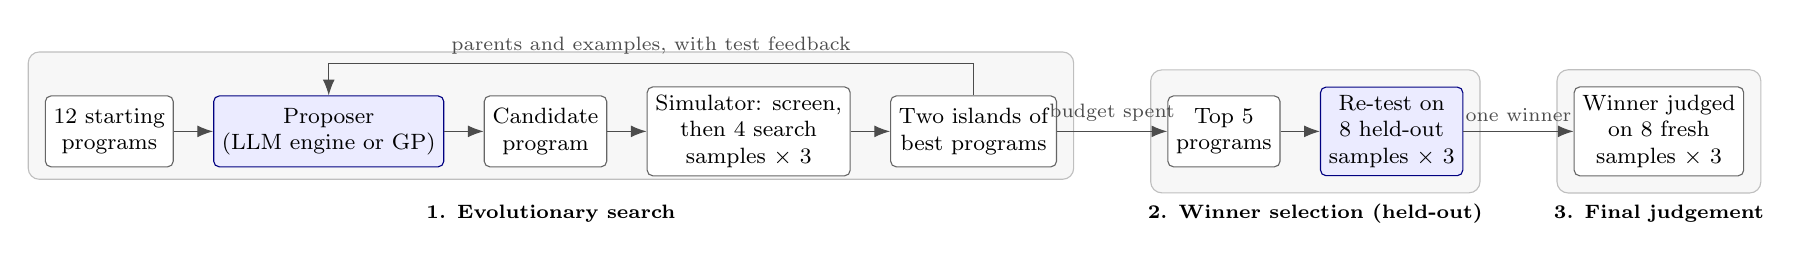
\begin{tikzpicture}[
  box/.style={draw=black!60, rounded corners=2pt, align=center, font=\footnotesize,
              minimum height=9mm, inner sep=3pt, fill=white},
  hl/.style={box, fill=blue!8, draw=blue!50!black},
  arr/.style={-{Latex[length=2mm]}, black!70},
  stage/.style={draw=black!25, fill=black!3, rounded corners=4pt, inner sep=6pt},
  node distance=5mm]
\node[box] (seed) {12 starting\\programs};
\node[hl, right=of seed] (prop) {Proposer\\(LLM engine or GP)};
\node[box, right=of prop] (cand) {Candidate\\program};
\node[box, right=of cand] (sim) {Simulator: screen,\\then 4 search\\samples $\times$ 3};
\node[box, right=of sim] (arch) {Two islands of\\best programs};
\node[box, right=14mm of arch] (top) {Top 5\\programs};
\node[hl, right=of top] (val) {Re-test on\\8 held-out\\samples $\times$ 3};
\node[box, right=14mm of val] (win) {Winner judged\\on 8 fresh\\samples $\times$ 3};
\draw[arr] (seed) -- (prop);
\draw[arr] (prop) -- (cand);
\draw[arr] (cand) -- (sim);
\draw[arr] (sim) -- (arch);
\draw[arr] (arch.north) -- ++(0,4mm) -| node[pos=0.25, above, font=\scriptsize]
  {parents and examples, with test feedback} (prop.north);
\draw[arr] (arch) -- node[above, font=\scriptsize]{budget spent}  (top);
\draw[arr] (top) -- (val);
\draw[arr] (val) -- node[above, font=\scriptsize]{one winner} (win);
\begin{scope}[on background layer]
\node[stage, fit=(seed)(arch)(prop.north), yshift=2mm, inner ysep=10pt] (s1) {};
\node[stage, fit=(top)(val)] (s2) {};
\node[stage, fit=(win)] (s3) {};
\end{scope}
% Stage labels share one baseline, set below the lowest stage boxes (s2, s3).
\coordinate (lab) at ([yshift=-9pt]s2.south);
\foreach \s/\t in {s1/1. Evolutionary search,
                   s2/2. Winner selection (held-out),
                   s3/3. Final judgement}
  \node[font=\scriptsize\bfseries, anchor=base] at (\s.south |- lab) {\t};
\end{tikzpicture}
\end{document}
